In this section we verify that, by construction, the optimal policy leads to the maximum success probability $P^{(L)}_*(\alpha)$.
It is assumed that $Q$ is always associated with the optimal policy $\pi^{*}$; we simplify notation by $Q = Q_{\pi^{*}}$.

At step $L$, given any history $h_{L}$, the actions available to the agent are $\hat{k} = a_L$, i.e. guessing for one of the possible phases of the coherent state. The Q-values at this time-step read as
\begin{equation}
  \begin{aligned}
  Q(h_{L}, a_L) = \mathbb{E}[G_L | h_L, a_L] &= \sum_{r_{L+1}} r_{L+1} \; p(r_{L+1}| h_L; a_L) \\
    &=  p( \alpha ^{(a_L)} | o_{1:L}, a_{0:(L-1)}) ,
  \end{aligned}
\end{equation}
with $o_{1:\ell} = \{o_1, o_2, ..., o_{\ell}\}$ the observations obtained up to the $\ell^{\text{\underline{th}}}$ photodetector, and $a_{0:\ell} = \{a_0, a_1 , ..., a_\ell \}$ the actions done up to step $\ell$. Such actions are deterministic functions of $h_\ell$, and thus we aim to optimize over all possible function choices (and for this reason we will here use the semi-colon notation in the probabilities).

Recalling that the optimal action, given $h_{\ell}$, is obtained from Q as $a^{*}(h_{\ell}) = \underset{a_{\ell}}{\text{argmax }} Q(h_\ell, a_\ell)$, the optimal guess $a_L^{*}$ is the one of maximum-likelihood:
\begin{equation*}
    a^{*}_L = \underset{a_L}{\text{argmax }} \; p( \alpha ^{(k)} | o_{1:L}; a_{0:(L-1)}) \Big|_{k=a_{L}}.
\end{equation*}

By definition of the optimal policy and because the optimal Bellman equation Eq.~\eqref{eq:qBellOp} holds, namely
\begin{eqnarray}
Q^{*}(s,a)&&:=Q_{\pi^*}(s,a)=\max_\pi Q_\pi(s,a)\\
&&=\sum_{s'\in\cS,r\in\cR}\tau(s',r|s,a)(r+\gamma \max_{a'\in\cA}Q^{*}(s',a')),
\end{eqnarray}
then the optimal action to take given history $h_{L-1}$ at step $L-1$ is
{\small
\begin{equation}\begin{aligned}
  &a^{*}_{L-1} = \underset{a_{L-1}}{\text{argmax }} \; Q(h_{L-1}, a_{L-1}) \\
  &= \underset{a_{L-1}}{\text{argmax }} \sum_{o_L} p(o_{L}|o_{1:(L-1)}; a_{0:(L-1)}) \; \max_{a_{L}}  \; Q(h_L, a_L) \\
  &= \underset{a_{L-1}}{\text{argmax }} \sum_{o_L} p(o_{L}|o_{1:(L-1)}; a_{0:(L-1)}) \; \max_{k} \; p( \alpha ^{(k)} | o_{1:L}; a_{0:(L-1)}) \\
  &= \underset{a_{L-1}}{\text{argmax }} \; \sum_{o_L}  \; \frac{\max_{k} \; p(o_{1:L} | \alpha ^{(k)}; a_{0:(L-1)}) p_k}{p(o_{1:(L-1)}; a_{0:(L-1)}) }, \\
\end{aligned}\end{equation}
}%
where in the last line we have used Bayes theorem. Following this line of reasoning, we can obtain the optimal actions $a^{*}_{\ell}$ at any time-step. In particular, for $\ell=0$, by recursively applying the optimal Bellman equation (Eq.~\eqref{eq:qBellOp}) we have
% % % %

\begin{eqnarray}\label{eq:OptQLL}
Q(h_0, a_0)&=& \sum_{o_1} p(o_1; a_0) \; \underset{a_1}{\max } \; Q(h_1, a_1)  \\ \nonumber
&=& \sum_{o_1} p(o_1; a_0) \; \underset{a_1}{\max } \; \sum_{o_{2}} p(o_{2}|o_{1}; a_1) \; \underset{a_2}{\max } \; Q(h_2, a_2) \\ \nonumber
& = &  \sum_{o_1} p(o_1; a_0) \; \underset{a_1}{\max } \sum_{o_{2}} p(o_{2}|o_{1}; a_1) \; \underset{a_2}{\max } \sum_{o_3} \; \Big( \\ \nonumber
& (...) & \; \sum_{o_{L}}  p(o_L|o_{1:(L-1)}; a_{1:(L-1)}) \; \underset{a_L}{\max}\; Q(h_L, a_L)\Big) \\  \nonumber
&=& \sum_{o_1} \; \underset{a_1}{\max } \sum_{o_{2}} \; \underset{a_2}{\max } \sum_{o_3} \; \Big( \\ \nonumber
& (...) & \; \sum_{o_{L}}  \; \underset{k}{\max}\; p(o_{1:L}|\alpha^{(k)}; a_{0:(L-1)}) \; p_k \Big). \\  \nonumber
\end{eqnarray}

Therefore, by taking the optimal action $a^{*}_0 = \underset{a_{0}}{\text{argmax }} Q(h_0,a_0)$, we obtain
\begin{equation}
  \underset{a_0}{\text{max }} Q(h_0,a_0) = p_*^{(L)},
\end{equation}
which was defined in Eq.~\ref{eq:32OptSuc}, though here we dropped the dependence on $\alpha$. As pointed out in the main text, the value and action-value functions are related via $v_\pi(s) = \sum_{a}\pi(a|s)Q_{\pi}(s,a)$. Therefore, the optimal value function for the initial state is the optimal success probability:
\begin{equation}
  v_*(h_0) = \sum_{a} \delta \big(a, \underset{a}{\text{argmax }} Q(h_0, a)) = Q(h_0, a^{*}_0 \big) = P_*^{L}(\alpha).
\end{equation}

In Fig.~\ref{fig:profiles} we show several sections of the estimats $\hat{Q}$, using 1-greedy as the interaction policy and each update made according $Q$-learning, at episode $t = 10^{8}$,

\begin{figure}[t]
    \centering
    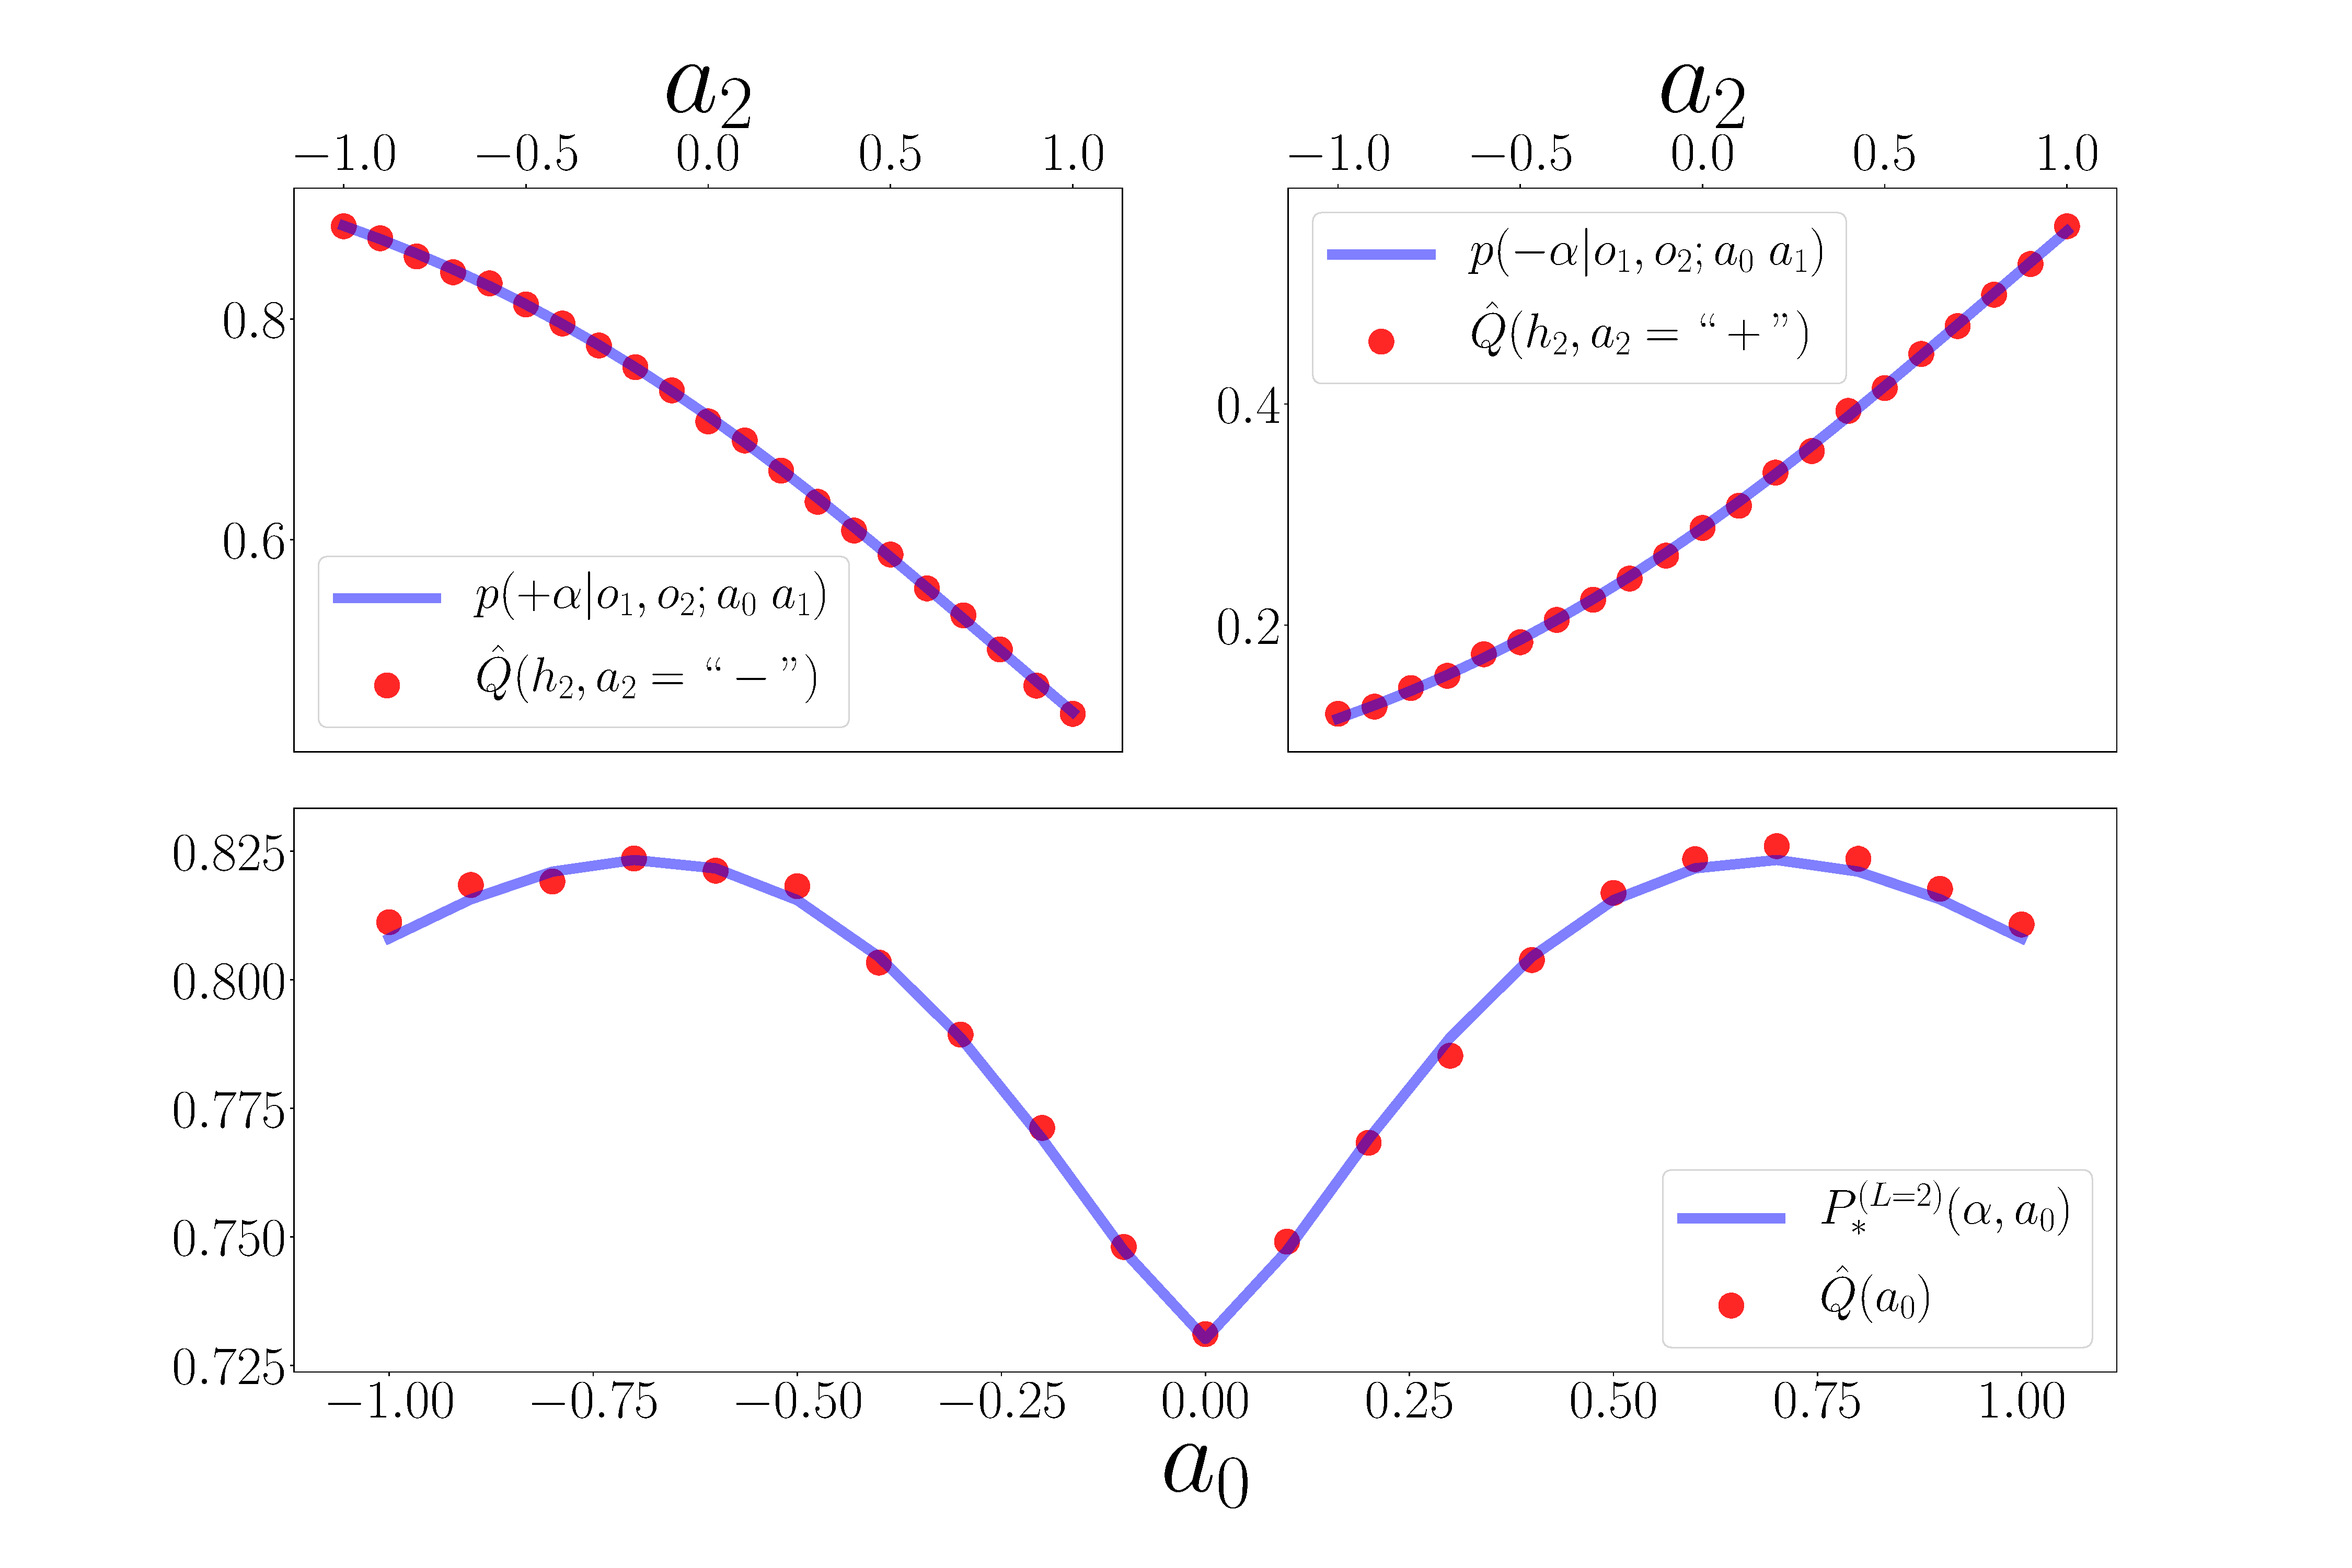
\includegraphics[width=1.\textwidth]{Figures/315/qprofguess108.pdf}
    \caption{We plot different values of the Q-estimates, after $10^{8}$ episodes of random exploration ($\epsilon = 1$), updating the Q-estimates according to Q-learning (see Algorithm 1). The random exploration is used in order to ensure that, at \textit{finite} number of episodes, all state-action pairs were equally visited on average. The lower plot corresponds to the estimates $\hat{Q}(a_0)$, and it is compared with the optimal success probability as a function of $a_0$, i.e. $P_*^{(L=2)}(\alpha, a_0) =  \sum_{o1}\;p(o_1; a_0) \; \underset{a_1}{\text{max}} \sum_{o_2} p(o_2|h_1, a_1) \; \underset{a_2 = \pm}{\text{max }} p(\pm \alpha | h_2) pr(\pm \alpha)$.}
    \label{fig:profiles}
\end{figure}

The success of $Q$-learning agents in finding the optimal configurations of Dolinar-like receivers crucially depends on accurately estimating the success probability of the relevant configurations. Such configurations correspond to the \textit{interesting} region of the state-action space (\textit{i.e.} where high rewards are allocated), and as we have seen, they are related to optimal state-action value functions $Q^*$.

From such optimal values, the agent can straightfowardly follow an optimal policy $\pi^*$ by going greedy with respect to them. Nevertheless, as we stressed in Sec.~\ref{ssec:1_rl_seqDec}, learning begins without the knowledge of how to access those high-rewarding configurations, and hence the agent needs to balance between exploring new ones (through displacements that has not been performed previously) and performing displacements that have previously led to a reward of $1$ with a high probability. In the latter case, statistical fluctuations when estimating success probabilities out of measurement outcomes can potentially hide the fact that some displacements are actually sub-optimal. To balance such trade-off, $Q$-learning selects a displacement according to an $\epsilon$-greedy strategy.

As introduced in Sec.~\ref{ssec:1_rl_bandit}, bandit theory defines the so-called regret, that precisely captures the \textit{exploration-exploitation} tradeoff in Markov Reward Processes. In that Section, we introduced strategies based on Upper Confidence Bounds (UCB) or Thompson Sampling (TS) which outperforms $\epsilon$-greedy ones in terms of the expected regret. It is thus sensible to ask wheter the $Q$-learning agent can be enhanced with such bandit-based strategies, and hence we now turn to study how these enhanced agents perform in our BPSK coherent-state discrimination problem.
%
